\documentclass[11pt, oneside]{article}   	% use "amsart" instead of "article" for AMSLaTeX format
\usepackage{geometry}                		% See geometry.pdf to learn the layout options. There are lots.
\geometry{letterpaper}                   		% ... or a4paper or a5paper or ... 
%\geometry{landscape}                		% Activate for for rotated page geometry
%\usepackage[parfill]{parskip}    		% Activate to begin paragraphs with an empty line rather than an indent
\usepackage{graphicx}				% Use pdf, png, jpg, or eps� with pdflatex; use eps in DVI mode
								% TeX will automatically convert eps --> pdf in pdflatex		
\usepackage{amssymb}
\usepackage{amsmath}
\usepackage{parskip}

\title{Polar Coordinates}
%\author{The Author}
%\section{}
% \subsection*{R code}
\date{}							% Activate to display a given date or no date

\graphicspath{{/Users/telliott_admin/Dropbox/Tex/png/}}

\begin{document}
\maketitle
\Large
%\noindent

Standard polar coordinates plots points in terms of distance from the origin, $r$ and the angle that this ray makes with the positive $x$-axis, $\theta$.  Converting from $x,y$ to $r, \theta$ is pretty easy:

\[ x = r \cos \theta \]
\[ y = r \sin \theta \]

To go the other way, use Pythagoras to write 

\[ x^2 + y^2 = r^2 \]
\[ \theta = \tan^{-1} (\frac{y}{x}), \ \ x \ne 0 \]

In polar coordinates, as in Cartesian ($xy$) coordinates, the equation of a circle depends on whether it is at the origin or not.  If it is at the origin, then something like

\[ r = 3 \]

defines the graph.  But if it's not, then the equations are of the form:

\[ r = a \cos \theta + b \sin \theta \]

For example, 

\[ r = 3 \sin \theta \]

is a circle centered at $x = 0, y = 3/2$, with a radius of $3/2$ (it passes through the origin and the point $(x=0,y=3)$.

while

\[ r = \sin \theta + \cos \theta \]

is a circle centered at  $x = 3/2, y = 3/2$ which passes through the origin.

Let's see if we can manipulate these equations to go back to Cartesian coordinates.

\[ r = 3 \sin \theta \]
\[ y = r \sin \theta \]
\[ \sin \theta = \frac{y}{r} \]
\[ r = \frac{3y}{r} \]
\[ r^2 = 3y = x^2 + y^2 \]
complete the square:
\[ x^2 + y^2 -3y + \frac{3}{2} =  \frac{3}{2} \]
\[ x^2 + (y - \frac{3}{2})^2 = (\sqrt{\frac{3}{2}})^2 \]

Similarly,

\[ r = \sin \theta + \cos \theta \]
\[ r = \frac{y}{r} + \frac{x}{r} \]
\[ r^2 = x + y = x^2 + y^2 \]
\[ x^2 - x + \frac{1}{4} + y^2 - y + \frac{1}{4} = \frac{1}{2} \]
\[ (x - \frac{1}{2})^2 + (y - \frac{1}{2})^2 = (\frac{1}{\sqrt{2}})^2 \]

One can also write the equations for other conic sections in polar coordinates.  For example, the following is a parabola:

\[ r = \frac{2}{1 + \sin \theta} \]

Plot it to see.  Or just do this:

\[ r  + r \sin \theta) = 2 \]
\[ \frac{y}{r} = \sin \theta \]
\[ r + y = 2 \]
\[ r^2 = (2-y)^2  = x^2 + y^2 \]
\[ 4 - 4y + y^2 = x^2 + y^2 \]
\[ y - 1 = -\frac{1}{4} x^2  \]

The next page has some examples from \emph{The Calculus Lifesaver}.

\begin{center} 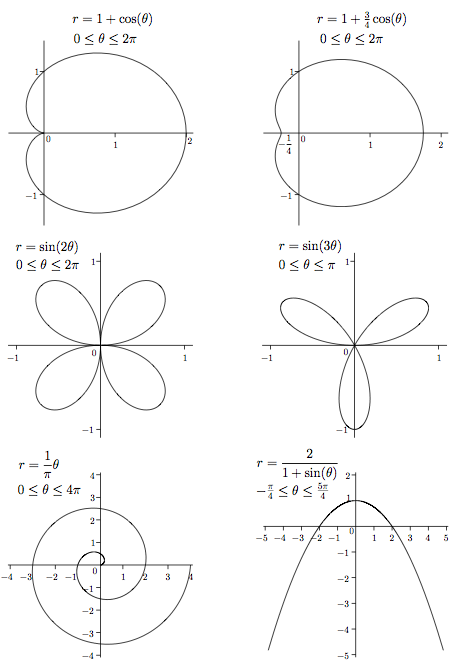
\includegraphics [scale=0.75] {polarex.png} \end{center}

\subsection*{Integration to find areas}

The idea for (one-dimensional) integration in polar coordinates is that we know $r$ as a function of $\theta$.  For example, we had the circle centered at $(0,3/2)$ given by

\[ r = 3 \sin \theta \]

We imagine dividing up the circle into little triangles, sectors where 

\[ \theta \rightarrow \theta + \Delta \theta \]

The sector is approximately a triangle with side $r$ and base $r \times \Delta \theta$ (the latter is the length of the arc of the circle on its circumference).

The area of each little sector is

\[ \frac{1}{2} r^2 d \theta \]
\subsection*{example}
For this problem:
\[ r = 3 \sin \theta \]

The total area is then
\[ \int_0^{2\pi}  \frac{1}{2} r^2 d \theta \]
\[ = \int_0^{2\pi}  \frac{1}{2} (3 \sin \theta)^2 d \theta \]
\[ = \frac{9}{2} \int_0^{2\pi}  \sin^2 \theta d \theta \]

This looks hard but we've done it before.  One way is to recall that 

\[ [ \ \sin \theta \cos \theta \ ]' = - \sin^2 \theta + \cos^2 \theta \]
\[ =  1 - 2 \sin^2 \theta \]
Integrate
\[ \int [ \ \sin \theta \cos \theta \ ]' \ d \theta = \int (1 - 2 \sin^2 \theta) \ d \theta \]
\[ \sin \theta \cos \theta  = \theta - 2 \int \sin^2 \theta \ d \theta \]
Hence
\[ \int \sin^2 \theta \ d \theta = \frac{1}{2}  (\theta - \sin \theta \cos \theta) \]

So our answer is

\[ = (\frac{9}{2}) \ \frac{1}{2} (x -  \sin \theta \cos \theta) \ \bigg |_0^{2\pi} \]
\[ =  (\frac{9}{2}) \ \frac{1}{2} (2 \pi) \]
\[ = \frac{9\pi}{4} \]

which is correct for a circle with radius $3/2$.
\subsection*{example}
The second example is from \emph{How to ace the rest of calculus}.  We have two circles, both of radius $1$.  The first one is centered at the origin.  We are given the equation of the second in polar coordinates:
\[ r = 2 \cos \theta \]
Plugging in some values for $\theta$: and calculating $r$:
\[ \theta = 0 \rightarrow r = 2 \]
\[ \theta = \frac{\pi}{6} \rightarrow r = \frac{\sqrt{3}}{2} \]
\[ \theta = \frac{\pi}{4} \rightarrow r = \sqrt{2} \]
\[ \theta = \frac{\pi}{3} \rightarrow r = 1 \]
\[ \theta = \frac{\pi}{2} \rightarrow r = 0 \]

We can also convert to $x,y$-coordinates.  Multiply by $r$:
\[ r^2 = 2 r \cos \theta \]
Substituting $r^2 = x^2 + y^2$ and $x = r \cos \theta$:
\[ x^2 + y^2 = 2x \]
Complete the square:
\[ (x^2 - 2x + 1) + y^2 = 1 \]
\[ (x-1)^2 + y^2 = 1 \]
The second circle is centered at $(1,0)$.  Note that for this circle it is \emph{not} true that $x^2 + y^2 = 1$.

Now, the problem given is to calculate the shaded area in the figure.
\begin{center} 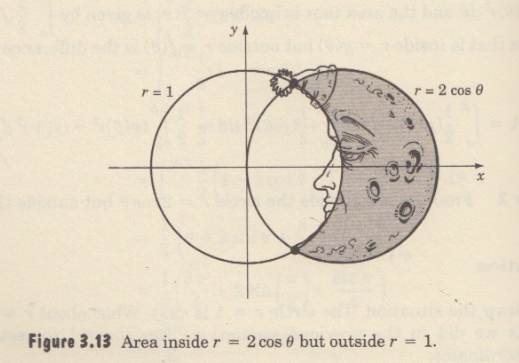
\includegraphics [scale=0.5] {two-circles.png} \end{center}
First, we must find the value of $\theta$ at the points of intersection between the two circles.  We solve the two equations simultaneously:
\[ y^2 = 1 - x^2 \]
\[ (x - 1)^2 + y^2 =  (x - 1)^2 + 1 - x^2 = 1 \]
\[ -2x + 2 = 1 \]
\[ 2x = 1 \]
\[ x = \frac{1}{2} \]
\[ y = \sqrt{1 - x^2} = \pm \frac{\sqrt{3}}{2} \]
\[ \theta = \tan^{-1} \frac{y}{x} = \pm \sqrt{3} \]
Look it up:
\[ \theta = \pm \frac{\pi}{3} \]
or notice that we are on the unit circle so $\cos \theta = x = 1/2$, $\theta = \pm \pi/3$.
That's the hard way.  The easy way is
\[ r = 1 = 2 \cos \theta \]
\[ \theta = \cos^{-1} \frac{1}{2} = \frac{\pi}{3} \]

The area of an arc of the unit circle is the $r^2$ times one-half the arc length in radians.
\[ A = \frac{1}{2} \ \int r^2 \ d \theta \]
We will subtract the area of the inner arc from that covered by the outer one
\[ A = \frac{1}{2} \int_{-\pi/3}^{\pi/3} (2 \cos \theta)^2 - 1 \ d \theta \]
Recall that
\[ \cos 2 \theta = \cos^2 \theta - \sin^2 \theta = \cos^2 \theta - 1 + \cos^2 \theta \]
\[ \cos^2 \theta = \frac{1}{2} (1 + \cos 2 \theta) \]
so
\[ (2 \cos \theta)^2 = 4 \ \frac{1}{2} (1 + \cos 2 \theta) = 2(1 + \cos 2 \theta) \]
\[ A = \frac{1}{2} \int_{-\pi/3}^{\pi/3} (2 \cos \theta)^2 - 1 \ d \theta \]
\[ = \frac{1}{2} \int_{-\pi/3}^{\pi/3} 2 \cos 2 \theta + 1 \ d \theta \]
\[ = \frac{1}{2} \ [ \ \sin 2 \theta + \theta \ ] \ \bigg |_{-\pi/3}^{\pi/3} \]
Since $\sin 2 \pi / 3 = \sqrt{3}/2$:
\[ = \frac{1}{2} (\sqrt{3} + \frac{2 \pi}{3}) = \frac{\sqrt{3}}{2} + \frac{\pi}{3} \]
\subsection*{example}
\begin{center} 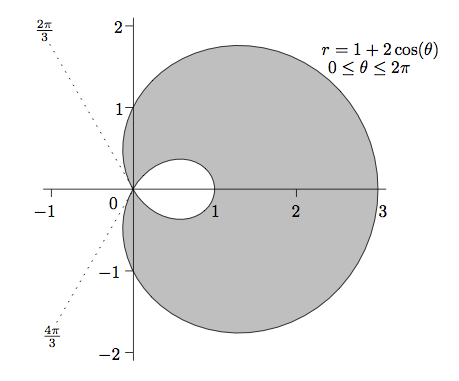
\includegraphics [scale=0.5] {cardioid.png} \end{center}
Recall

\[ A = \int  \frac{1}{2} r^2 d \theta \]

so plug in to obtain

\[ \int  \frac{1}{2} (1 + 2 \cos \theta)^2 d \theta \]
\[ \int  \frac{1}{2} (1 + 4 \cos \theta + 4 \cos^2 \theta) d \theta \]
\[ = \frac{\theta}{2} + 2 \sin \theta + 2\int cos^2 \theta + C \]

We've already done both $\cos^2 \theta$) and $\sin^2 \theta$ above.  Since we already have the integral for $\sin^2$, and to approach things a bit differently, recall

\[ \sin^2 \theta + \cos^2 \theta = 1 \]
Hence
\[ \int \sin^2 \theta \ d\theta + \int \cos^2 \theta \ d\theta = \int 1 \ d\theta \]
So
\[ \int \cos^2 \theta \ d\theta = \theta - \ [ \ \frac{1}{2}  (\theta - \sin \theta \cos \theta) \ ] \]
\[ = \frac{1}{2} ( \theta + \sin \theta \cos \theta) \]

Putting it all together, we obtain the expression:

\[ \frac{3}{2}\theta + 2 \sin \theta + \sin \theta \cos \theta \]

The cardioid is a strange shape.  We can get the area of the first sector ($\theta = 0 \rightarrow \pi/2$) easily, just evaluate the expression at both limits and subtract one from the other:

The $\sin \theta \cos \theta$ term goes away for both $\theta=0$ and $\theta = \pi/2$, as do all the other terms for $\theta = 0$, so we have just $2 + 3\pi/4$ as the area under the curve in the first quadrant.

On the other hand, if we look carefully at the figure and the equation, what happens as $\theta = \pi/2 \rightarrow \pi $?

\begin{center} 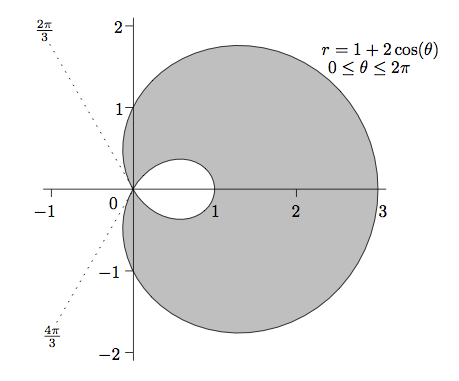
\includegraphics [scale=0.5] {cardioid.png} \end{center}

The part of the area that shows up as gray in the second quadrant comes comes between $\theta = \pi/2 \rightarrow 2\pi/3$.  We obtain that upper limit by solving for

\[ r = 1 + 2 \cos \theta = 0 \]
\[ \cos \theta = - \frac{1}{2}  \]

The angle with cosine - 1/2 in this quadrant is $2\pi/3$.

So now we need to evaluate the expression at $\theta = 2\pi/3$:
\[ \frac{3}{2}\theta + 2 \sin \theta + \sin \theta \cos \theta \]
\[ \pi + \sqrt{3} - \frac{\sqrt{3}}{4} = \pi + \frac{3}{4}\sqrt{3} \]

This (minus the value at $\pi/2$) is the area of the sliver in the second quadrant.  (And notice, we could never do this in Cartesian coordinates).

The last part is even weirder.  If you follow the graph it comes into the fourth quadrant and arches up to the point $(1,0)$, when $\theta = \pi$.  How can this be?  It happens because although $\theta = 2\pi/3 \rightarrow \pi$ ($\theta$ is still in the second quadrant), the value of $r$ is \emph{negative}.  

In order to get the whole area, we will integrate between $\theta = 0 \rightarrow 2\pi$, but we would like to count the part of the area between $\theta = 2/3 \pi \rightarrow 4/3 \pi$ as negative, subtracting it from the earlier result (see the picture).  The problem is that our formula has $r^2$ in it.  We fix that by doing the calculation but remembering the area is really negative.  

Further we need to subtract this funny area twice ..

The reason is that the area we get by integrating ($\theta = 0 \rightarrow 2\pi$) is really this:

\begin{center} 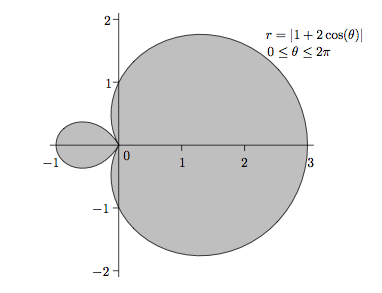
\includegraphics [scale=0.75] {cardioid2.png} \end{center}


At $\theta = 4/3 \pi$

\[ \frac{3}{2}\theta + 2 \sin \theta + \sin \theta \cos \theta \]
\[ 2\pi - \sqrt{3} + \frac{\sqrt{3}}{4} = 2 \pi - \frac{3}{4} \sqrt{3} \]


In summary, we have these values for our expression

\[ f(0)=0 \]
\[  f(\frac{1}{2}\pi ) = 2 + \frac{3}{4} \pi \]
\[  f(\frac{2}{3}\pi ) = \pi + \frac{3}{4}\sqrt{3} \]
\[  f(\pi ) = \frac{3}{2}\pi \]
\[ f(\frac{4}{3}\pi ) = 2\pi - \frac{3}{4} \sqrt{3} \]
\[  f(2\pi ) = 3 \pi \]

So the total is 

\[ 3 \pi - 0 - 2\ [ \ (2\pi - \frac{3}{4} \sqrt{3}) - (\pi + \frac{3}{4}\sqrt{3}) \ ]  \]
\[ = 3 \pi - 2(\pi - \frac{3}{2} \sqrt{3}) \]
\[ = \pi + 3 \sqrt{3} \approx 8.38 \]

Compare that with the area of a circle of radius $1/2$, $\approx 7.07$.  It looks like a reasonable answer.

\subsection*{Arc length}

I think this is more a problem for Calculus BC but I saw it on the web and got interested, and the answer turns out to be particularly simple, so let's take a look.  Suppose we have this equation

\[ r = \sin^2 \frac{\theta}{2} \]

I don't have the greatest intuition for these things yet, but a plot shows this is a cardioid.

\begin{center} 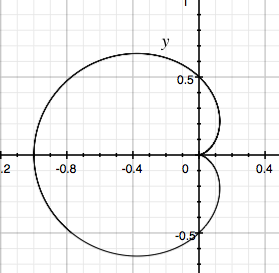
\includegraphics [scale=0.75] {arc_cardioid.png} \end{center}

The problem asks us to find the \emph{arc length}.  If this were a problem in Cartesian coordinates, we would be looking for each little bit of arc length $ds$ which is the hypotenuse of a right triangle with sides $dx$ and $dy$ and so

\[ ds^2 = dx^2 + dy^2 \]

Multiply and divide on the right by $dx^2$

\[ ds^2 = (1 + (\frac{dy}{dx})^2) \ dx^2 \]
\[ ds = \sqrt{1 + (\frac{dy}{dx})^2} \ dx \]

We just integrate this from the starting point to the end point.

What about polar coordinates?  If you sketch what happens along a little bit of arc of a curve in polar coordinates, one side of our right triangle is $dr$, but the other side is $r d\theta$ ($\theta$ by itself is just an angle).  So

\[ ds^2 = r^2 d \theta^2 + dr^2 \]

Multiply and divide on the right by $d\theta^2$
\[ ds^2 = (r^2 + (\frac{dr}{d \theta})^2)) \ d \theta^2 \]
\[ ds = \sqrt{r^2 + (\frac{dr}{d \theta})^2} \ d \theta \]

Check it in wikipedia to confirm.  OK.

Returning to the function in the problem

\[ r = \sin^2 \frac{\theta}{2} \]
\[ r^2 = \sin^4 \frac{\theta}{2} \]
\[ \frac{dr}{d\theta} = 2 \sin \frac{\theta}{2} (\frac{1}{2}) \cos  \frac{\theta}{2}  \]
\[ = \sin \frac{\theta}{2} \cos  \frac{\theta}{2}  \]
\[ (\frac{dr}{d\theta})^2 = \sin^2 \frac{\theta}{2} \cos^2  \frac{\theta}{2}  \]

So
\[ ds = \sqrt{\sin^4 \frac{\theta}{2} + \sin^2 \frac{\theta}{2} \cos^2  \frac{\theta}{2}} \ d \theta \]
\[ = \sin \frac{\theta}{2} \sqrt{\sin^2 \frac{\theta}{2} +  \cos^2  \frac{\theta}{2}} \ d \theta \]
\[ = \sin \frac{\theta}{2}  \ d \theta \]

To get the arc length we integrate $ds$

\[ \int \ ds = - 2 \cos \frac{\theta}{2} + C \]

For example from $\theta = 0 \rightarrow \pi$

\[  = - 2 \cos \frac{\theta}{2} \ \bigg |_0^{\pi} = 2 \]

which seems reasonable.  If this were a circle with radius $r=0.5$, the semi-perimeter would be $\pi r \approx 1.57$.



\end{document}  